\documentclass{beamer}
% Ceci est mon powerpoint pour l'atelier du 14 mai 2019
\usepackage[backend=biber]{biblatex}
\addbibresource{RQC.bib}
\usepackage{amsfonts}
\usepackage{amssymb}
\usepackage{amsthm}
\usepackage{amsmath}
\usepackage{amsopn} 
\usepackage[T1]{fontenc}
\usepackage[utf8]{inputenc}
\UseRawInputEncoding
\usepackage{url}
\usepackage{multicol}
\uselanguage{French}
\languagepath{French}
\usepackage{pgf}
\usepackage{tikz}
\usepackage{graphicx}
\usepackage[french]{babel}
\mode<presentation> {
\usetheme{Madrid}}
\usecolortheme{default}
\useoutertheme{default}
\setbeamercovered{transparent}
\beamertemplatenavigationsymbolsempty
\definecolor{ulrouge}{RGB}{254,51,0}
\definecolor{ulor}{RGB}{254,204,0}
\definecolor{noir}{RGB}{0,0,0}
\setbeamercolor{palette primary}{bg=ulor,fg=noir}
\setbeamercolor{palette secondary}{bg=ulrouge,fg=noir}
\setbeamercolor{palette tertiary}{bg=ulrouge,fg=noir}
\setbeamercolor{palette quaternary}{bg=ulrouge,fg=noir}
\setbeamercolor{structure}{fg=noir} % itemize, enumerate, etc
\setbeamercolor{section in toc}{fg=noir} % TOC sections
\title{\textbf{Utilisation du paquet plm: application en relations industrielles}}
\author{\textbf{Mil\`ene R. E. Lokrou \\ \'Etudiante au doctorat en relations industrielles}} 
\institute{\textbf{Universit\'e Laval}}
\date{\textbf{14 mai 2019}}
\graphicspath{{figures/}}
\begin{document}
\setbeamertemplate{footline}[frame number]
\setbeamercolor*{section in head/foot}{bg=ulrouge,fg=noir}
\begin{frame}
\titlepage
	
\includegraphics[width=2cm]{RQC.png}\hfill
	
\includegraphics[width=4cm]{UL2.jpg}
\end{frame}
\begin{frame}
\frametitle{\textbf{Structure de l'atelier}}
\tableofcontents
\end{frame}
\section{\textbf{Introduction}}
\subsection{Rappel: donn\'ees de panel}
\subsection{Estimation sur des donn\'ees de panel avec R}
\subsection{Objectifs de l'atelier}
\begin{frame}{\textbf{Introduction}}
\setbeamercolor{block title}{use=structure,bg=noir,fg=white}
\setbeamercolor{block body}{use=structure,bg=ulor,fg=noir}
\begin{block}{Rappel: donn\'ees de panel}
\end{block}
Les donn\'ees dites de panel renferment deux dimensions: 
\begin{enumerate}
\item Des donn\'ees transversales
\item Des s\'eries temporelles
\end{enumerate}
\end{frame}
\begin{frame}{\textbf{Introduction}}
\setbeamercolor{block title}{use=structure,bg=noir,fg=white}
\setbeamercolor{block body}{use=structure,bg=ulor,fg=noir}
\begin{block}{Rappel: donn\'ees de panel}
\end{block}
Avantages li\'es  \`a l'utilisation de donn\'ees de panel:
\begin{enumerate}
\item Meilleur contr\^ole de l'h\'et\'erog\'en\'eit\'e
\item Donn\'ees plus riches d'informations 
\item Possibilit\'e de capter certaines dynamiques 
\item Capacit\'e de produire des analyses plus complexes 
\end{enumerate}
\end{frame}
\begin{frame}{\textbf{Introduction}}
\setbeamercolor{block title}{use=structure,bg=noir,fg=white}
\setbeamercolor{block body}{use=structure,bg=ulor,fg=noir}
\begin{block}{Rappel: donn\'ees de panel}
\end{block}
Dans un panel typique, le nombre d'individus n est grand et celui des
p\'eriodes T est petit. \newline

Cependant, un panel peut pr\'esenter une ou plusieurs caract\'eristiques (Park, 2011): 
\begin{itemize}
\item court 
\item long 
\item cylindr\'e
\item non cylindr\'e 
\item fixe 
\item rotatif 
\end{itemize}
\end{frame}
\begin{frame}{\textbf{Introduction}}
\setbeamercolor{block title}{use=structure,bg=noir,fg=white}
\setbeamercolor{block body}{use=structure,bg=ulor,fg=noir}
\begin{block}{Rappel: donn\'ees de panel}
\end{block}
\begin{figure}
\begin{center}
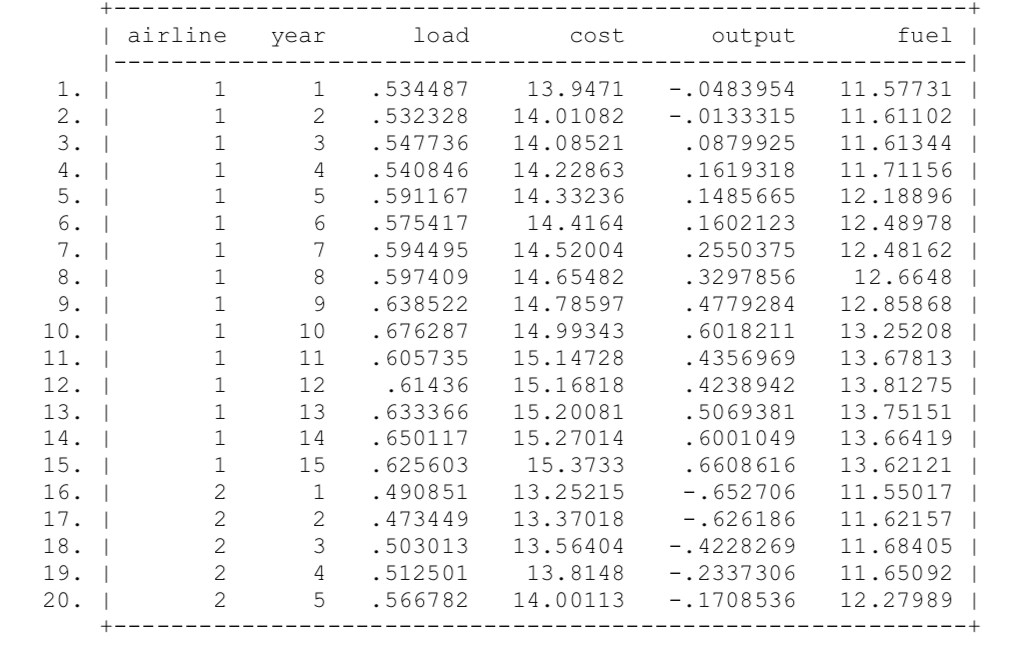
\includegraphics [width=9cm] {Panel.png} 
\end{center}
\caption{exemple de donn\'ees de panel (Source: Park, 2011, p. 4)}
\label{exemple de donn\'ees de panel (Source: Park, 2011, p. 4)}
\end{figure}
\end{frame}
\begin{frame}{\textbf{Introduction}}
\setbeamercolor{block title}{use=structure,bg=noir,fg=white}
\setbeamercolor{block body}{use=structure,bg=ulor,fg=noir}
\begin{block}{Estimation sur des donn\'ees de panel avec R}
\end{block}
Dans R, plusieurs paquets permettent de produire une estimation sur des donn\'ees de panel. On peut citer, entre autres, les paquets: 
\begin{itemize}
\item phtt (pour l'effet de temps);
\item splm (pour des donn\'ees spatiales);
\item lme4 (pour les mod\`eles lin\'eaires mixtes);
\item nlme (pour les mod\`eles lin\'eaires et non lin\'eaires mixtes);
\item plm (pour les mod\`eles lin\'eaires). 
\end{itemize}
\end{frame}
\begin{frame}{\textbf{Introduction}}
\setbeamercolor{block title}{use=structure,bg=noir,fg=white}
\setbeamercolor{block body}{use=structure,bg=ulor,fg=noir}
\begin{block}{Objectifs de l'atelier}
\end{block}
Dans le cadre de cet atelier, nous allons utiliser le paquet plm. Quatre objectifs sont par ailleurs vis\'es: 
\begin{enumerate}
\item Pr\'esenter le paquet plm et l'int\'er\^et de celui-ci
\item Offrir une analyse de donn\'ees de panel sur la base d'un cas pratique
\item Sp\'ecifier les mod\`eles ad\'equats (tests de sp\'ecification)
\item Estimer des mod\`eles \`a  effets fixes et \`a  effets al\'eatoires
\end{enumerate} 
\end{frame}
\section{\textbf{Les mod\`eles lin\'eaires}}
\begin{frame}{\textbf{Les mod\`eles lin\'eaires}}
\setbeamercolor{block title}{use=structure,bg=noir,fg=white}
\setbeamercolor{block body}{use=structure,bg=ulor,fg=noir}
Tel que mentionn\'e par  Brigitte Dormont (1989, p.20), <<le choix le plus fr\'equent en \'econom\'etrie des donn\'ees de panel consiste \`a adopter une sp\'ecification en terme de mod\`ele  \`a erreurs compos\'ees>>. \newline

\begin{block}{Regression lin\'eaire simple}
Le cas simple d'un mod\`ele d'analyse de donn\'ees de panel \`a une seule variable explicative (x) peut donc \^etre sp\'ecifi\'e comme suit: 
    \begin{equation*}
y_{it}=x_{it}b + u_{it}
    \end{equation*}
\end{block}
avec i = 1, \ldots , N et t = 1, \ldots ,T 
et le terme d'erreur $u_{it} = \alpha_i + \varepsilon_{it}$
\end{frame}
\begin{frame}{\textbf{Les mod\`eles lin\'eaires}}
\setbeamercolor{block title}{use=structure,bg=noir,fg=white}
\setbeamercolor{block body}{use=structure,bg=ulor,fg=noir}
\begin{block}{Regression lin\'eaire simple}
Le cas simple d'un mod\`ele d'analyse de donn\'ees de panel \`a une seule variable explicative (x) peut donc \^etre sp\'ecifi\'e comme suit: 
    \begin{equation*}
y_{it}=x_{it}b + u_{it}
    \end{equation*}
\end{block}
O\`u: 
\begin{description} 
\item[i est une unit\'e statistique commun\'ement appel\'ee individu] 
\item[t est la p\'eriode]
\item[$x_{it}$ est la variable ind\'ependante et b la pente]
\item[$\alpha_i$ et $\varepsilon_{it}$ sont des perturbations al\'eatoires non corr\'el\'ees, d'esp\'erances nulles.]
\end{description}
\end{frame}
\section{\textbf{Pr\'esentation du paquet plm}}
\subsection{La structure des donn\'ees}
\subsection{Les mod\`eles d'estimation et l'interface}
\subsection{L'approche logicielle pour estimer}
\begin{frame}{\textbf{Pr\'esentation du paquet plm}}
\setbeamercolor{block title}{use=structure,bg=noir,fg=white}
\setbeamercolor{block body}{use=structure,bg=ulor,fg=noir}
\begin{block}{La structure des donn\'ees}
\end{block}
Dans R, l'identification d'une base de donn\'ees va reposer sur  un \textbf{data frame}. \newline

<<Un \textbf{data frame} est une liste de classe  \textbf{data.frame} dont tous les \'el\'ements sont de la m\^eme longueur (ou comptent le m\^eme nombre de lignes si les \'el\'ements sont des matrices).>> (Goulet, 2016, p. 30). 
\end{frame}
\begin{frame}{\textbf{Pr\'esentation du paquet plm}}
\setbeamercolor{block title}{use=structure,bg=noir,fg=white}
\setbeamercolor{block body}{use=structure,bg=ulor,fg=noir}
\begin{block}{La structure des donn\'ees}
\end{block}
Puisque les donn\'ees de panel renferment  deux dimensions (i.e.\ individuelle et temporelle). un argument \textbf{index} doit \^etre ajout\'e afin d'indiquer la structure des donn\'ees. Cet argument peut prendre quatre formes (Croissant et Millo, 2008):
\begin{enumerate}
\item NULL
\item Une cha\^ine de caract\`eres
\item Un vecteur de deux cha\^ines de caract\`eres
\item Un entier
\end{enumerate} 
\end{frame}
\begin{frame}{\textbf{Pr\'esentation du paquet plm}}
\setbeamercolor{block title}{use=structure,bg=noir,fg=white}
\setbeamercolor{block body}{use=structure,bg=ulor,fg=noir}
\begin{block}{Les mod\`eles d'estimation et l'interface}
\end{block}
4 mod\`eles d'estimation sont fournis par le paquet plm (Croissant et Millo, 2008, p.5):
\begin{enumerate}
\item plm: l'estimation classique des donn\'ees de panel. Dans ce mod\`ele, la fonction lm est utilis\'ee pour transformer les donn\'ees. 
\item pvcm: l'estimation des mod\`eles avec des coefficients variables. 
\item pgmm: l'estimation avec la m\'ethode des moments g\'en\'eralis\'ee.
\item pggls: l'estimation avec des moindres carr\'es g\'en\'eralis\'es faisables.
\end{enumerate} 
\end{frame}
\begin{frame}{\textbf{Pr\'esentation du paquet plm}}
\setbeamercolor{block title}{use=structure,bg=noir,fg=white}
\setbeamercolor{block body}{use=structure,bg=ulor,fg=noir}
\begin{block}{Les mod\`eles d'estimation et l'interface}
\end{block}
3 arguments sont communs aux mod\`eles d'estimation pr\'ec\'edents:
\begin{enumerate}
\item  l'index: i et t pour chaque observation
\item  l'effet: les effets individuels, les effets temporels ou les deux
\item  le mod\`ele : \`a effets fixes ou \`a effets al\'eatoires
\end{enumerate} 
\end{frame}
\begin{frame}{\textbf{Pr\'esentation du paquet plm}}
\setbeamercolor{block title}{use=structure,bg=noir,fg=white}
\setbeamercolor{block body}{use=structure,bg=ulor,fg=noir}
\begin{block}{L'approche logicielle pour estimer}
\end{block}
Comment obtenir un paquet plm qui fonctionne?
\begin{enumerate}
\item  \'Etape 1: t\'el\'echargez \textit{RStudio Desktop} (\url{https://www.rstudio.com/products/rstudio/download/}). 
\item  \'Etape 2: Installez les paquets plm, lmtest, zoo, formula, formula.tools. 
\end{enumerate} 
\end{frame}
\begin{frame}{\textbf{Pr\'esentation du paquet plm}}
\setbeamercolor{block title}{use=structure,bg=noir,fg=white}
\setbeamercolor{block body}{use=structure,bg=ulor,fg=noir}
\begin{block}{L'approche logicielle pour estimer}
\end{block}
Si le paquet formula est pr\'ealablement install\'e, vous pourrez avoir acc\`es au paquet plm en utilisant  la commande library("plm") dans Rstudio. \newline

Si vous n'avez aucun paquet install\'e, voici quelques captures d'\'ecran qui vous seront utiles pour les trouver, puis les installer. 
\begin{multicols}{3}
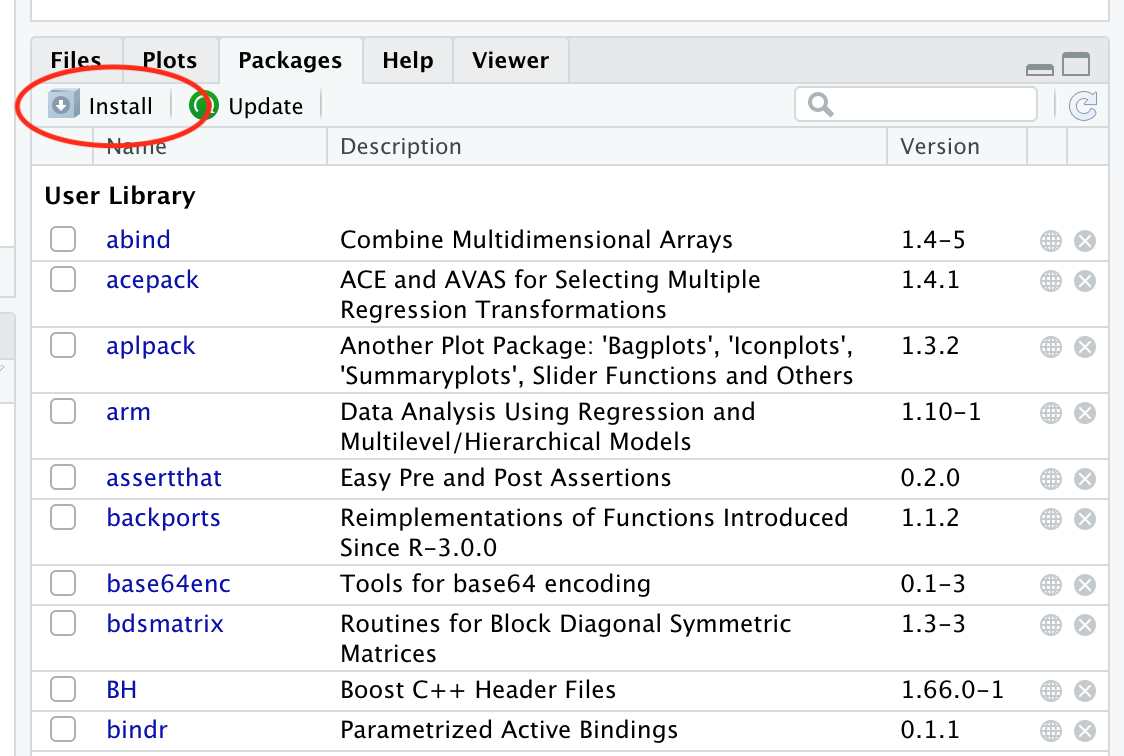
\includegraphics [width=4cm] {TrouverPackage.png} 
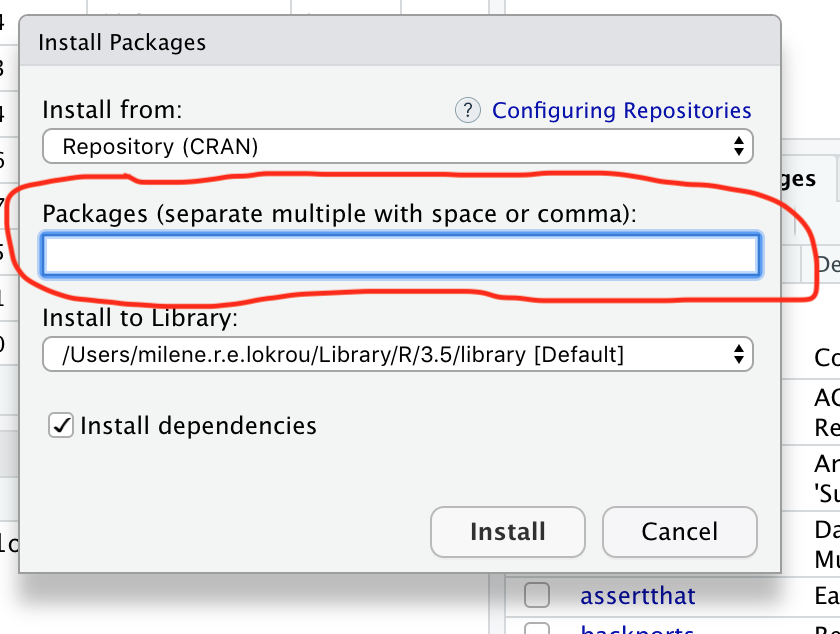
\includegraphics [width=4cm] {LUI.png} 
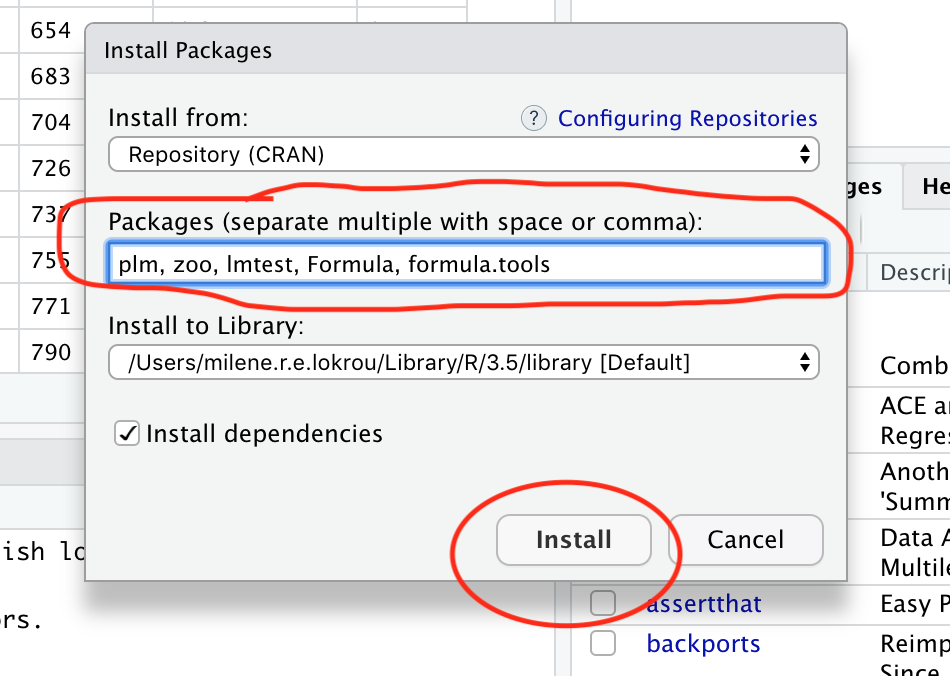
\includegraphics [width=4cm] {LUI2.png} 
\end{multicols}
\end{frame}
\begin{frame}{\textbf{Pr\'esentation du paquet plm}}
\setbeamercolor{block title}{use=structure,bg=noir,fg=white}
\setbeamercolor{block body}{use=structure,bg=ulor,fg=noir}
\begin{block}{L'approche logicielle pour estimer}
\end{block}
En fonction des arguments utilis\'es, le paquet plm permet d'estimer:
\begin{itemize}
\item Des effets fixes (within)
\item Des donn\'ees fusionn\'ees (pooling)
\item La premi\`ere diff\'erence (fd)
\item Les variations inter-individuelles (between)
\item Des mod\`eles \`a erreurs compos\'ees (random)
\end{itemize}
\end{frame}
\begin{frame}{\textbf{Pr\'esentation du paquet plm}}
\setbeamercolor{block title}{use=structure,bg=noir,fg=white}
\setbeamercolor{block body}{use=structure,bg=ulor,fg=noir}
\begin{block}{L'approche logicielle pour estimer}
\end{block}
L'utilisation g\'en\'erale du paquet plm consiste \`a indiquer la structure du mod\`ele, les donn\'ees et l'approche d'estimation choisie. \newline

Si l'on utilise des donn\'ees d\'ej\`a contenues dans r (e.g.\ data("Grunfeld", package = "Ecdat"), un usage basique du paquet plm \'equivaudra \`a:
\begin{itemize}
\item R> grun.fe <- plm(inv $\sim$ value + capital, data = Grunfeld, model = "within")
\item R> grun.re <- plm(inv $\sim$ value + capital, data = Grunfeld, model = "random")
\end{itemize}
\end{frame}
\begin{frame}{\textbf{Pr\'esentation du paquet plm}}
\setbeamercolor{block title}{use=structure,bg=noir,fg=white}
\setbeamercolor{block body}{use=structure,bg=ulor,fg=noir}
\begin{block}{L'approche logicielle pour estimer}
\end{block}
Il existe deux mod\`eles \`a erreurs compos\'ees: \newline

\textbf{\textit{Le mod\`ele \`a erreurs compos\'ees de type I}}
   \begin{equation*}
u_{it} = \alpha_i + \varepsilon_{it}
    \end{equation*}

\textbf{\textit{Le mod\`ele \`a erreurs compos\'ees de type II}}
   \begin{equation*}
u_{it} = \alpha_i + \lambda_t + \varepsilon_{it}
    \end{equation*}

  O\`u: 
\begin{description} 
 \item[$\lambda_t $ est l'effet inobserv\'e du temps]
\end{description} 
\end{frame}
\begin{frame}{\textbf{Pr\'esentation du paquet plm}}
\setbeamercolor{block title}{use=structure,bg=noir,fg=white}
\setbeamercolor{block body}{use=structure,bg=ulor,fg=noir}
\begin{block}{L'approche logicielle pour estimer}
\end{block}
Ces mod\`eles peuvent \^etre sp\'ecifi\'es dans le paquet plm. Par exemple, pour sp\'ecifier le mod\`ele de type II: \newline

R> grun.twfe <- plm(inv $\sim$ value + capital, data = Grunfeld, model = "within",
+    effect = "twoways") \newline

R> fixef(grun.twfe, effect = "time")
\end{frame}
\begin{frame}{\textbf{Pr\'esentation du paquet plm}}
\setbeamercolor{block title}{use=structure,bg=noir,fg=white}
\setbeamercolor{block body}{use=structure,bg=ulor,fg=noir}
\begin{block}{L'approche logicielle pour estimer}
\end{block}
Enfin, pour \'eviter des risques de mauvaise sp\'ecification des mod\`eles, plusieurs auteurs (e.g.\ Greene, 2011; Park, 2011) sugg\`erent l'utilisation de tests tels que celui de Hausman ou encore ceux du multiplicateur de Lagrange. 
\end{frame}
\begin{frame}{\textbf{Pr\'esentation du paquet plm}}
\setbeamercolor{block title}{use=structure,bg=noir,fg=white}
\setbeamercolor{block body}{use=structure,bg=ulor,fg=noir}
\begin{block}{L'approche logicielle pour estimer}
\end{block}
Pour le test de Hausman, \textbf{phtest} permet de l'ex\'ecuter. Les arguments principaux sont deux objets \textbf{panelmodel} ou une \textbf{formule}. Une application classique du test de Hausman consiste \`a comparer des mod\`eles \`a effets fixes et al\'eatoires. \newline

On aurait donc, en utilisant les donn\'ees Grunfeld  contenues dans le paquet plm:\newline

R> gw <- plm(inv $\sim$ value + capital, data = Grunfeld, model = "within") \newline

R> gr <- plm(inv $\sim$ value + capital, data = Grunfeld, model = "random") \newline

R> phtest(gw, gr)
\end{frame}
\begin{frame}{\textbf{Pr\'esentation du paquet plm}}
\setbeamercolor{block title}{use=structure,bg=noir,fg=white}
\setbeamercolor{block body}{use=structure,bg=ulor,fg=noir}
\begin{block}{L'approche logicielle pour estimer}
\end{block}
\textbf{plmtest} permet d'effectuer des tests du multiplicateur de Lagrange. L'argument principal est un objet \textbf{plm} auquel doivent imp\'erativement \^etre ajout\'es deux arguments en lien respectivement avec le type de test et les effets test\'es. On aurait donc, en utilisant les donn\'ees Grunfeld  contenues dans le paquet plm:\newline

R> g <- plm(inv $\sim$ value + capital, data = Grunfeld, model = "pooling")
R> plmtest(g, effect = "twoways", type = "bp") \newline

"bp" fait ici r\'ef\'erence au test de Breusch et Pagan. 
\end{frame}
\section{\textbf{Cas pratique: syndicalisation et ch\^omage aux \'Etats-Unis}}
\subsection{Description de la base de donn\'ees utilis\'ee}
\subsection{Application du paquet plm}
\begin{frame}{\textbf{Cas pratique: syndicalisation et ch\^omage aux \'Etats-Unis}}
\setbeamercolor{block title}{use=structure,bg=noir,fg=white}
\setbeamercolor{block body}{use=structure,bg=ulor,fg=noir}
\begin{block}{Description de la base de donn\'ees utilis\'ee}
\end{block}
\begin{itemize}
\item Les donn\'ees s'\'etendent de 2001 \`a 2017 et concernent 44 \'Etats am\'ericains. 
\item Notre base de donn\'ees contient donc n = 44 \'Etats and t = 18 ann\'ees. 
\item On assume que dans des \'Etats o\`u il y a un fort taux de syndicalisation, mesur\'e par le nombre de salari\'es membres d'un syndicat en pourcentage, il y a un faible taux de ch\^omage. 
\item On utilise comme variables de contr\^ole les salaires, les r\'egions (i.e.\ Nord-est, Sud, Mid-ouest, Ouest) et la crise de 2008-2009. 
\end{itemize}
\end{frame}
\begin{frame}{\textbf{Cas pratique: syndicalisation et ch\^omage aux \'Etats-Unis}}
Les r\'egions sont divis\'ees comme suit (Wilson, 2002, p. 9): 
\begin{figure}
\begin{center}
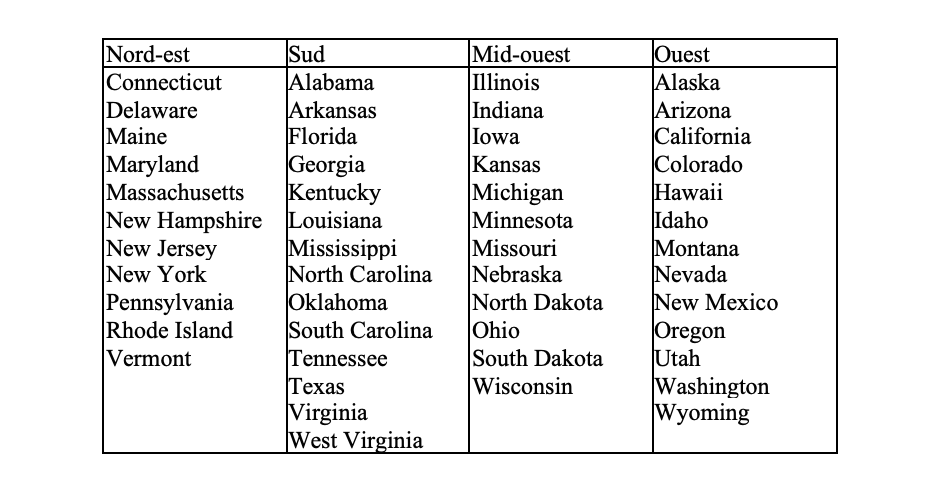
\includegraphics [width=10cm] {RUSA.png} 
\end{center}
\end{figure}
\end{frame}
\begin{frame}{\textbf{Cas pratique: syndicalisation et ch\^omage aux \'Etats-Unis}}
\setbeamercolor{block title}{use=structure,bg=noir,fg=white}
\setbeamercolor{block body}{use=structure,bg=ulor,fg=noir}
\begin{block}{Provenance des donn\'ees utilis\'ees}
\end{block}
\begin{itemize}
\item Local Area Unemployment Statistics (LAUS) (pour le taux de ch\^omage)
\item Quarterly Census of Employment and Wages (QCEW) (pour les salaires)
\item Current Population Survey (CPS) (pour la densit\'e syndicale)
\end{itemize}
\end{frame}
\begin{frame}{\textbf{Cas pratique: syndicalisation et ch\^omage aux \'Etats-Unis}}
\setbeamercolor{block title}{use=structure,bg=noir,fg=white}
\setbeamercolor{block body}{use=structure,bg=ulor,fg=noir}
\begin{block}{Application du paquet plm}
\end{block}
L'interface de RStudio, une fois les paquets utiles au bon fonctionnement du paquet plm install\'es, est le suivant: 
\begin{center}
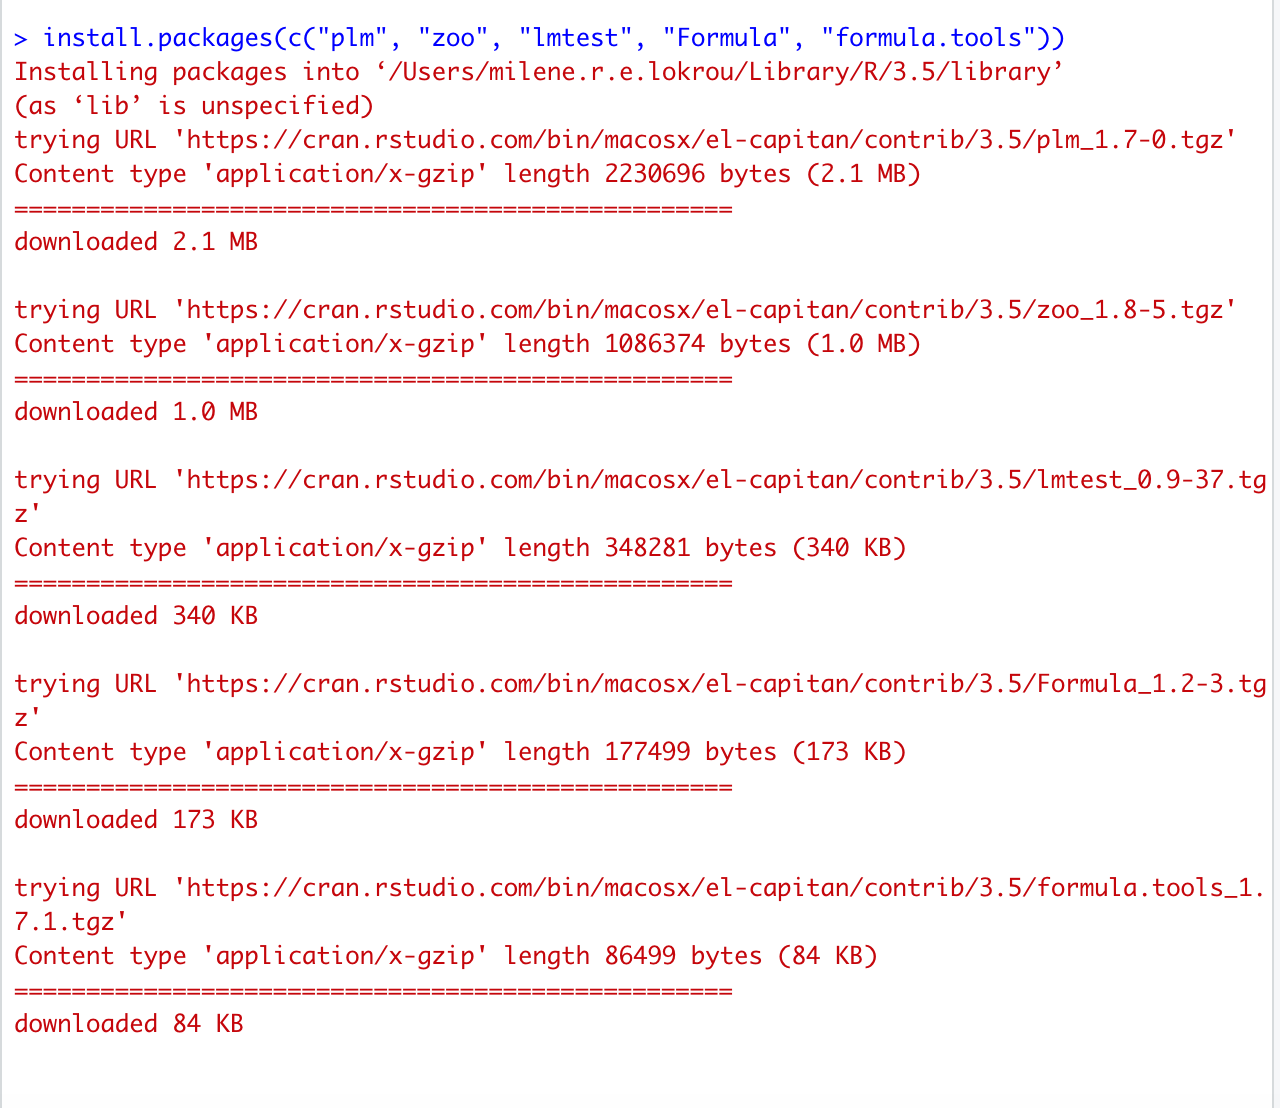
\includegraphics [width=7cm] {plmUtile.png} 
\end{center}
\end{frame} 
\begin{frame}{\textbf{Cas pratique: syndicalisation et ch\^omage aux \'Etats-Unis}}
\setbeamercolor{block title}{use=structure,bg=noir,fg=white}
\setbeamercolor{block body}{use=structure,bg=ulor,fg=noir}
\begin{block}{Application du paquet plm}
\end{block}
Pour commencer l'analyse des donn\'ees de panel, il  nous faut importer la base de donn\'ees \textbf{\textit{RAQC}} dans R. \newline

On peut importer une base de donn\'ees dans R de plusieurs mani\`eres. J'ai pour habitude de choisir \textbf{Excel}. 
\begin{multicols}{2}
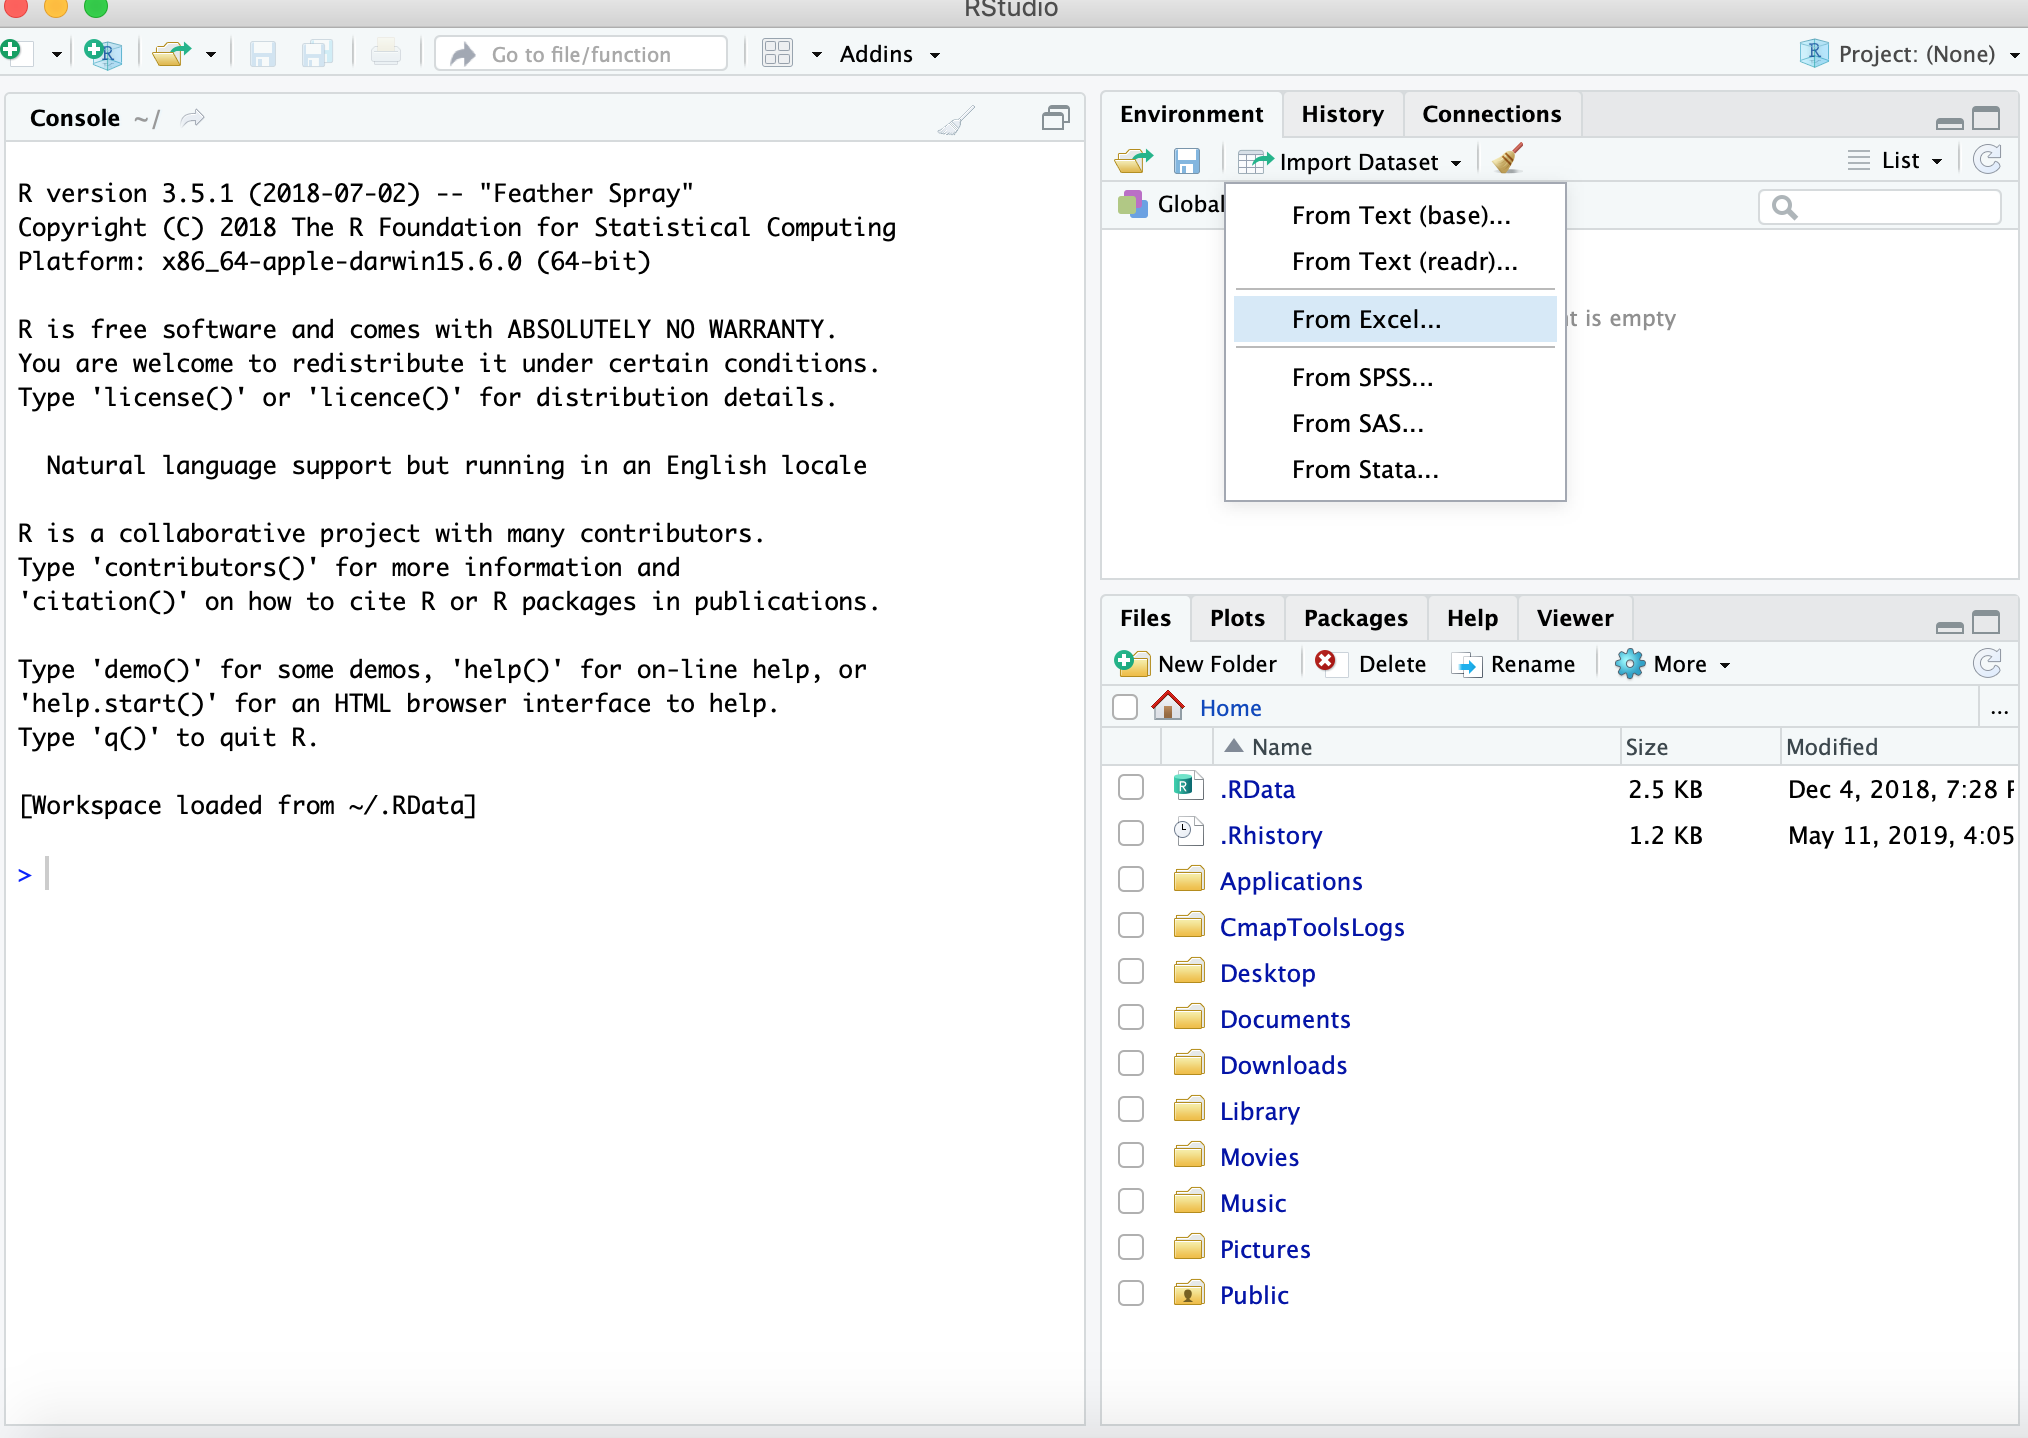
\includegraphics [width=5cm] {R2.png} 
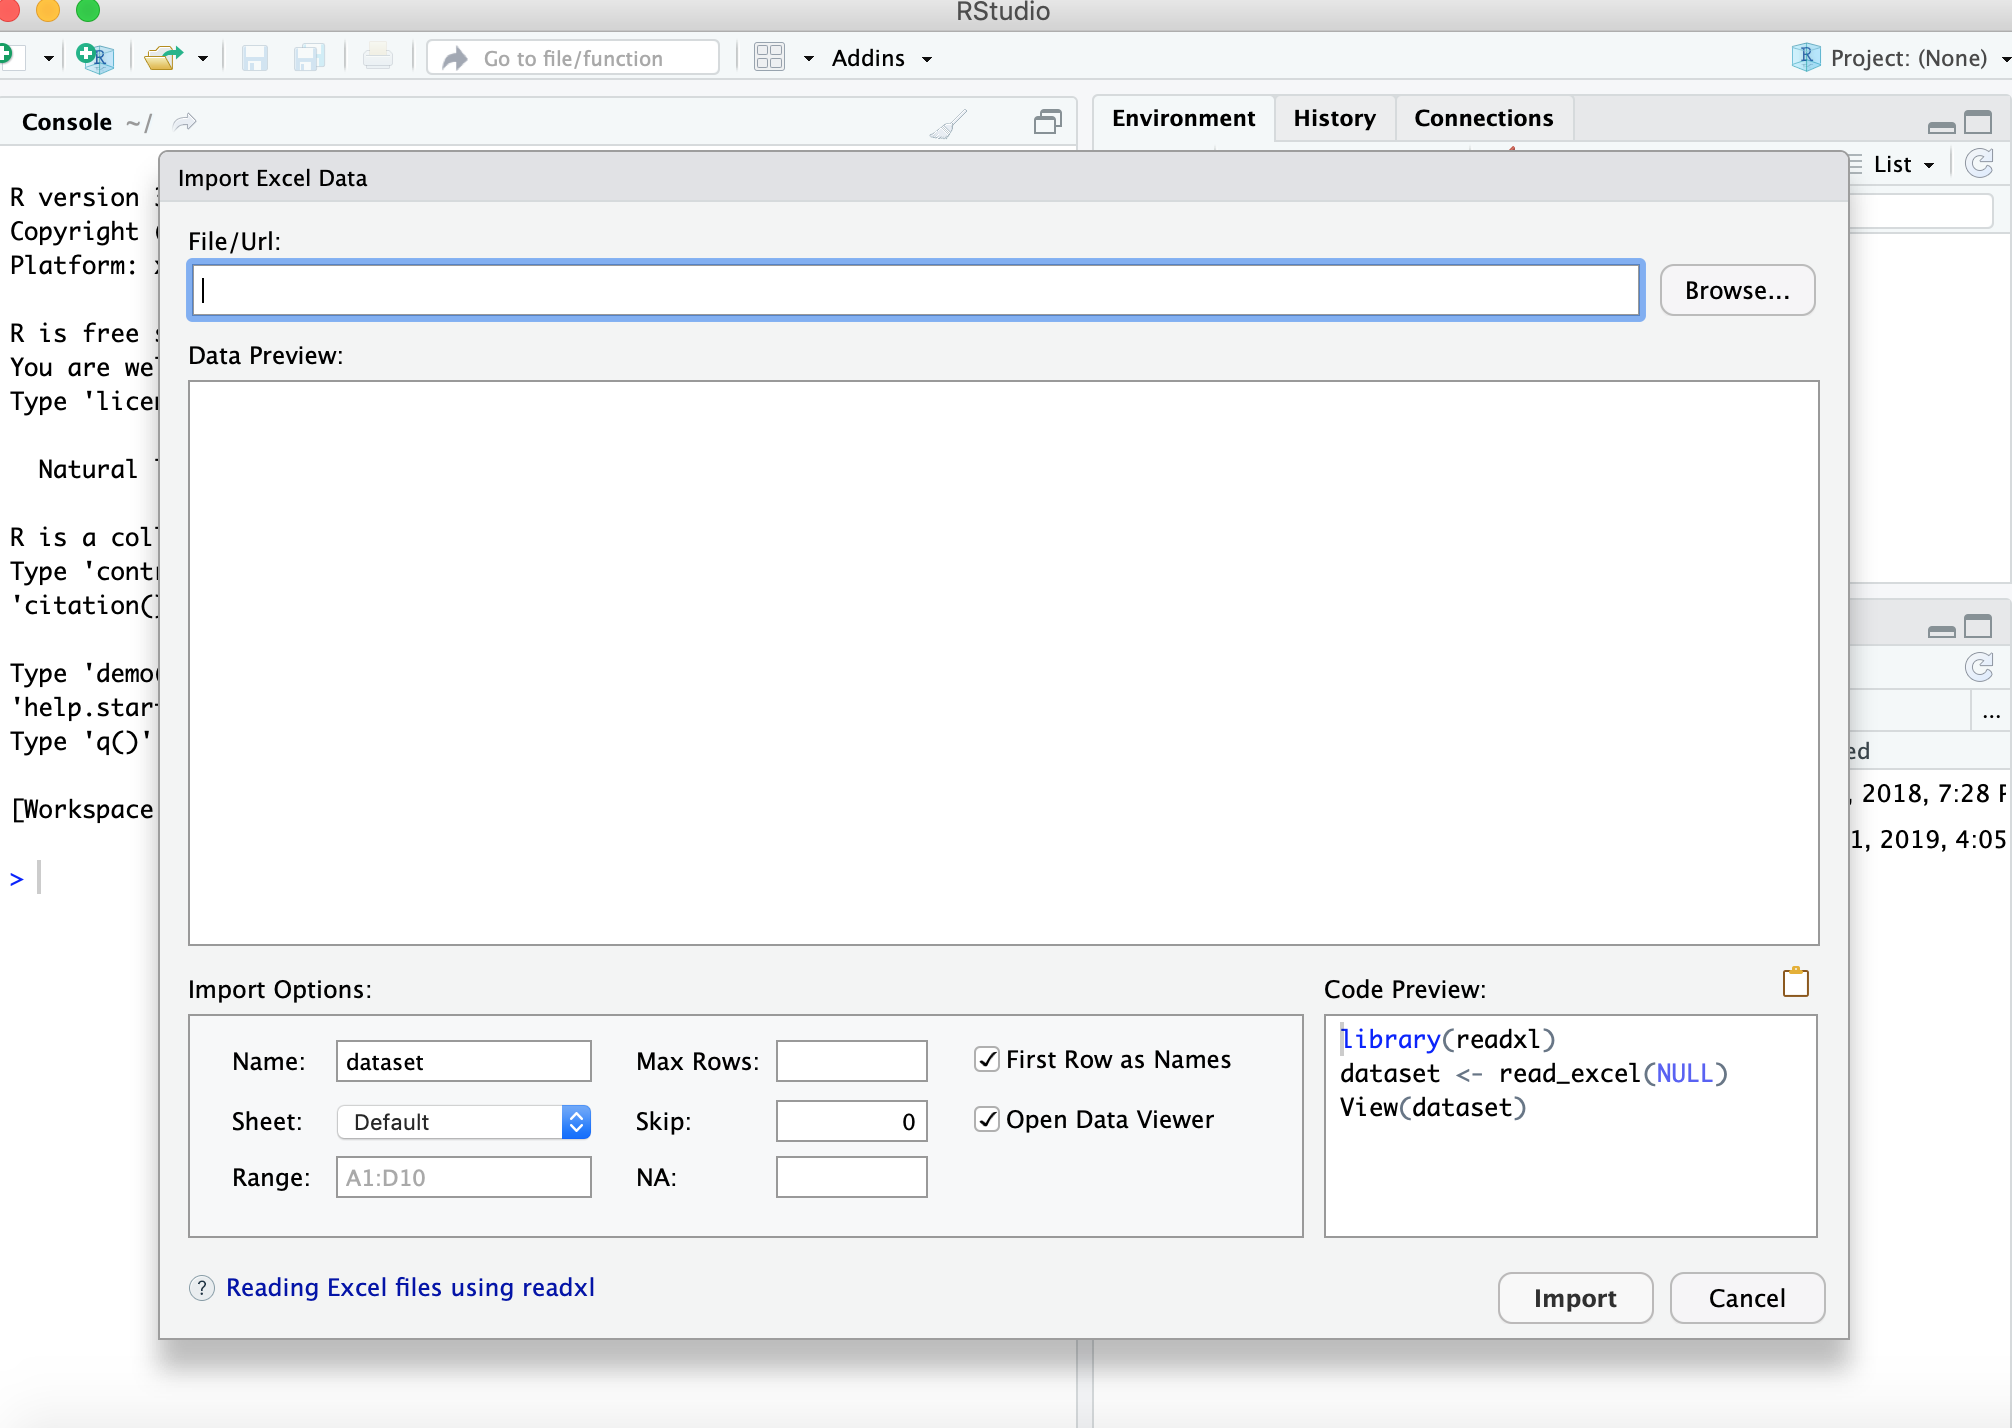
\includegraphics [width=5cm] {R1.png} 
\end{multicols}
\end{frame} 
\begin{frame}{\textbf{Cas pratique: syndicalisation et ch\^omage aux \'Etats-Unis}}
\setbeamercolor{block title}{use=structure,bg=noir,fg=white}
\setbeamercolor{block body}{use=structure,bg=ulor,fg=noir}
\begin{block}{Application du paquet plm}
\end{block}
Une fois la base de donn\'ees import\'ee, notre interface est la suivante: 
\begin{center}
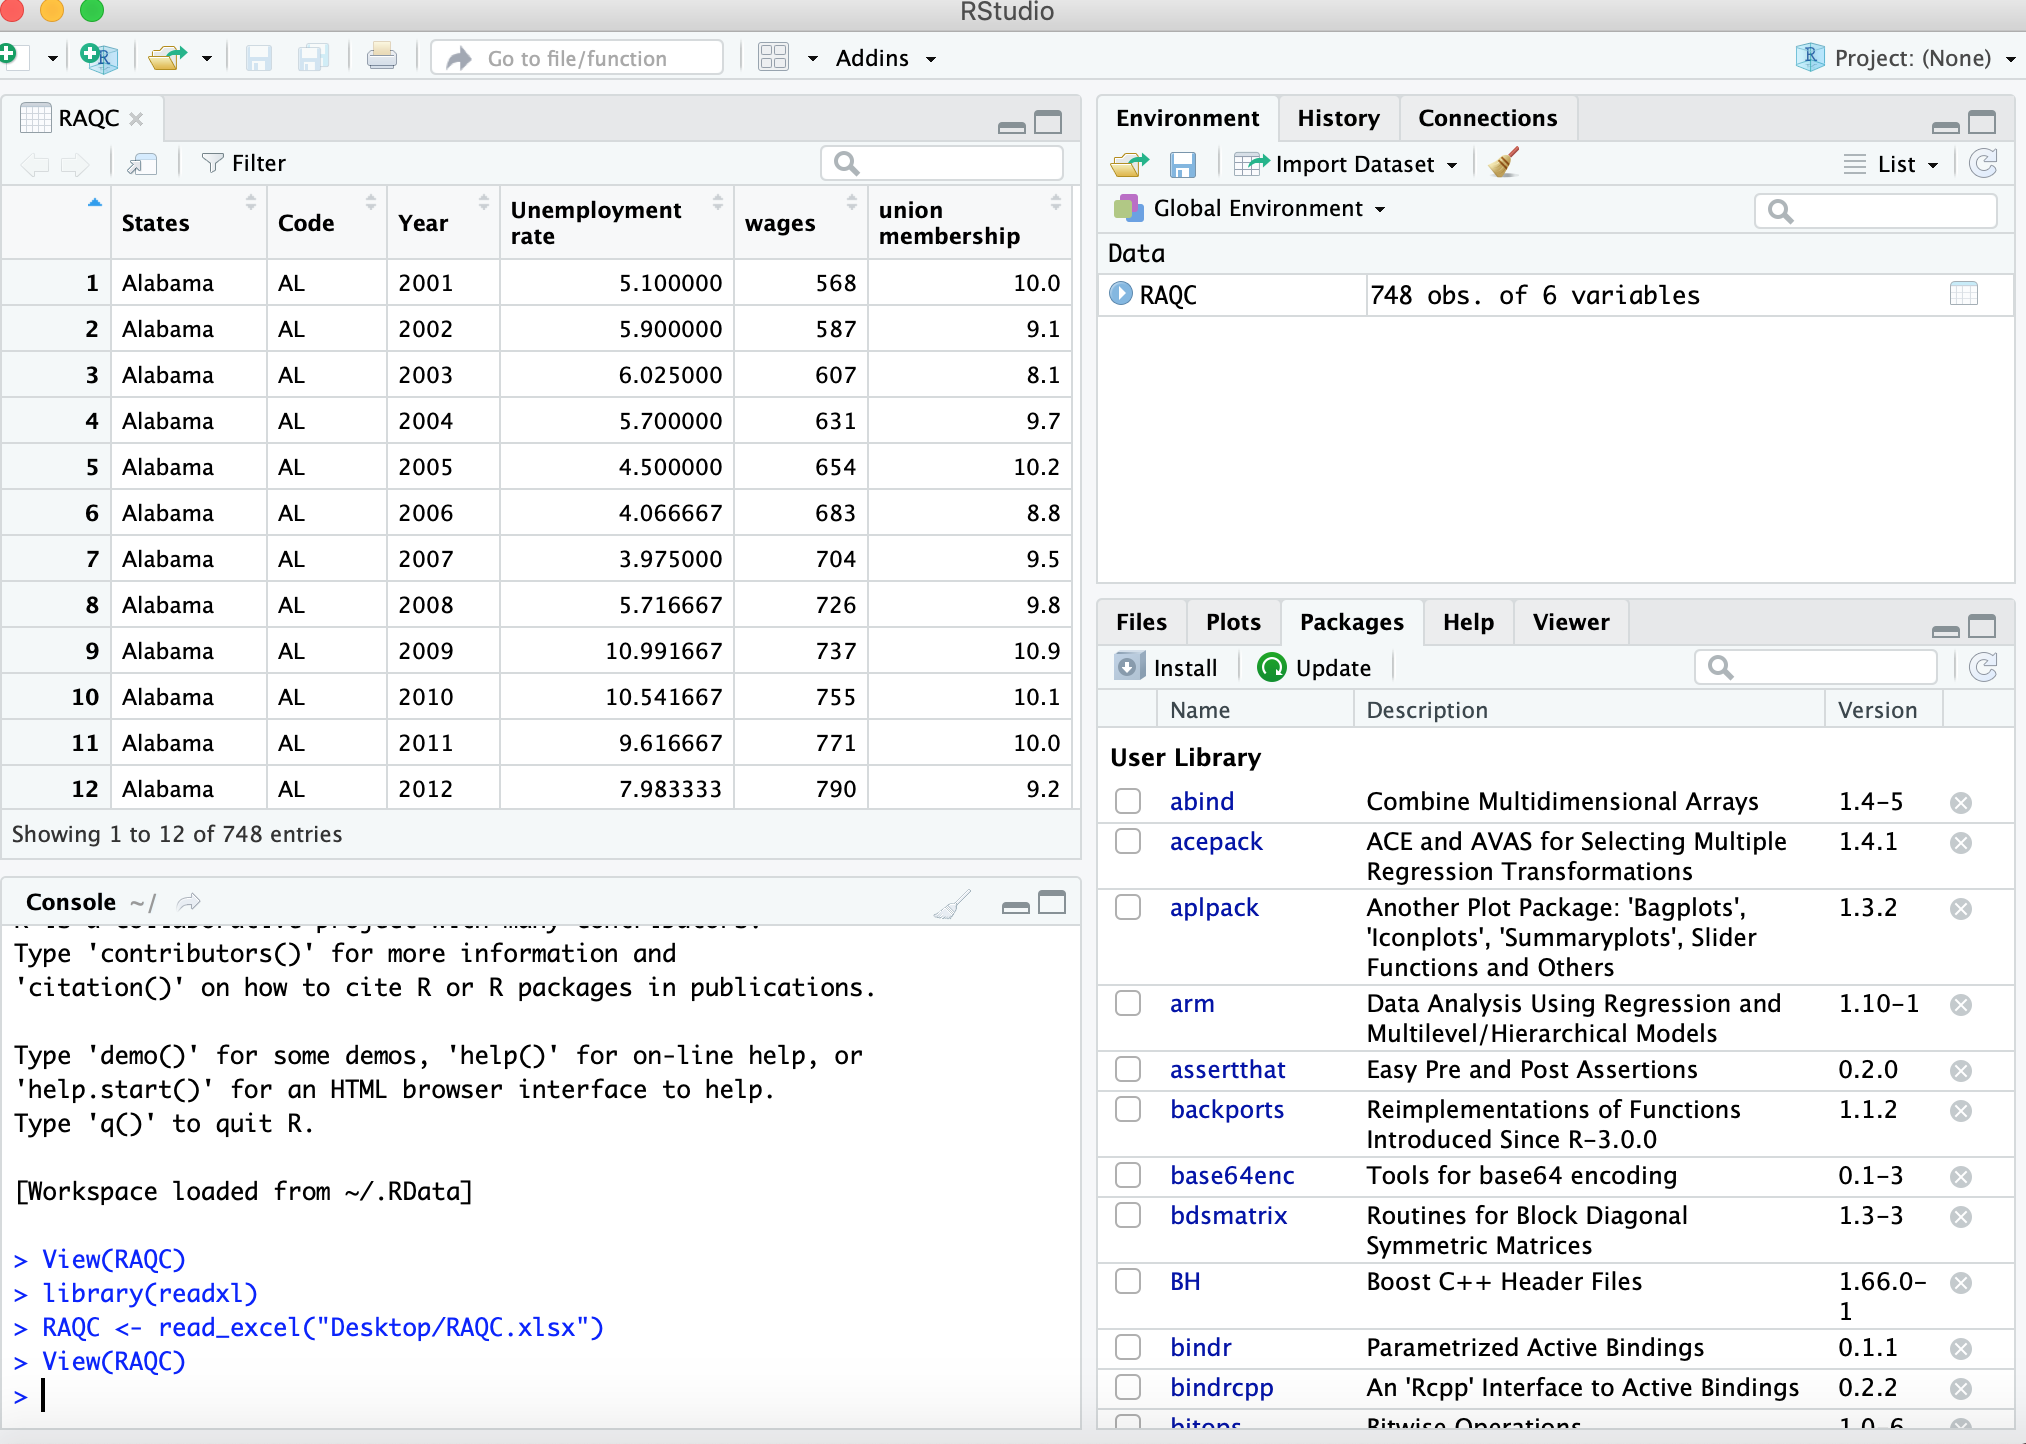
\includegraphics [width=8cm] {R3.png} 
\end{center}
\end{frame} 
\begin{frame}{\textbf{Cas pratique: syndicalisation et ch\^omage aux \'Etats-Unis}}
\setbeamercolor{block title}{use=structure,bg=noir,fg=white}
\setbeamercolor{block body}{use=structure,bg=ulor,fg=noir}
\begin{block}{Application du paquet plm}
\end{block}
On veut voir la structure de notre base de donn\'ees. On utilise la commande: \textbf{str}
\begin{center}
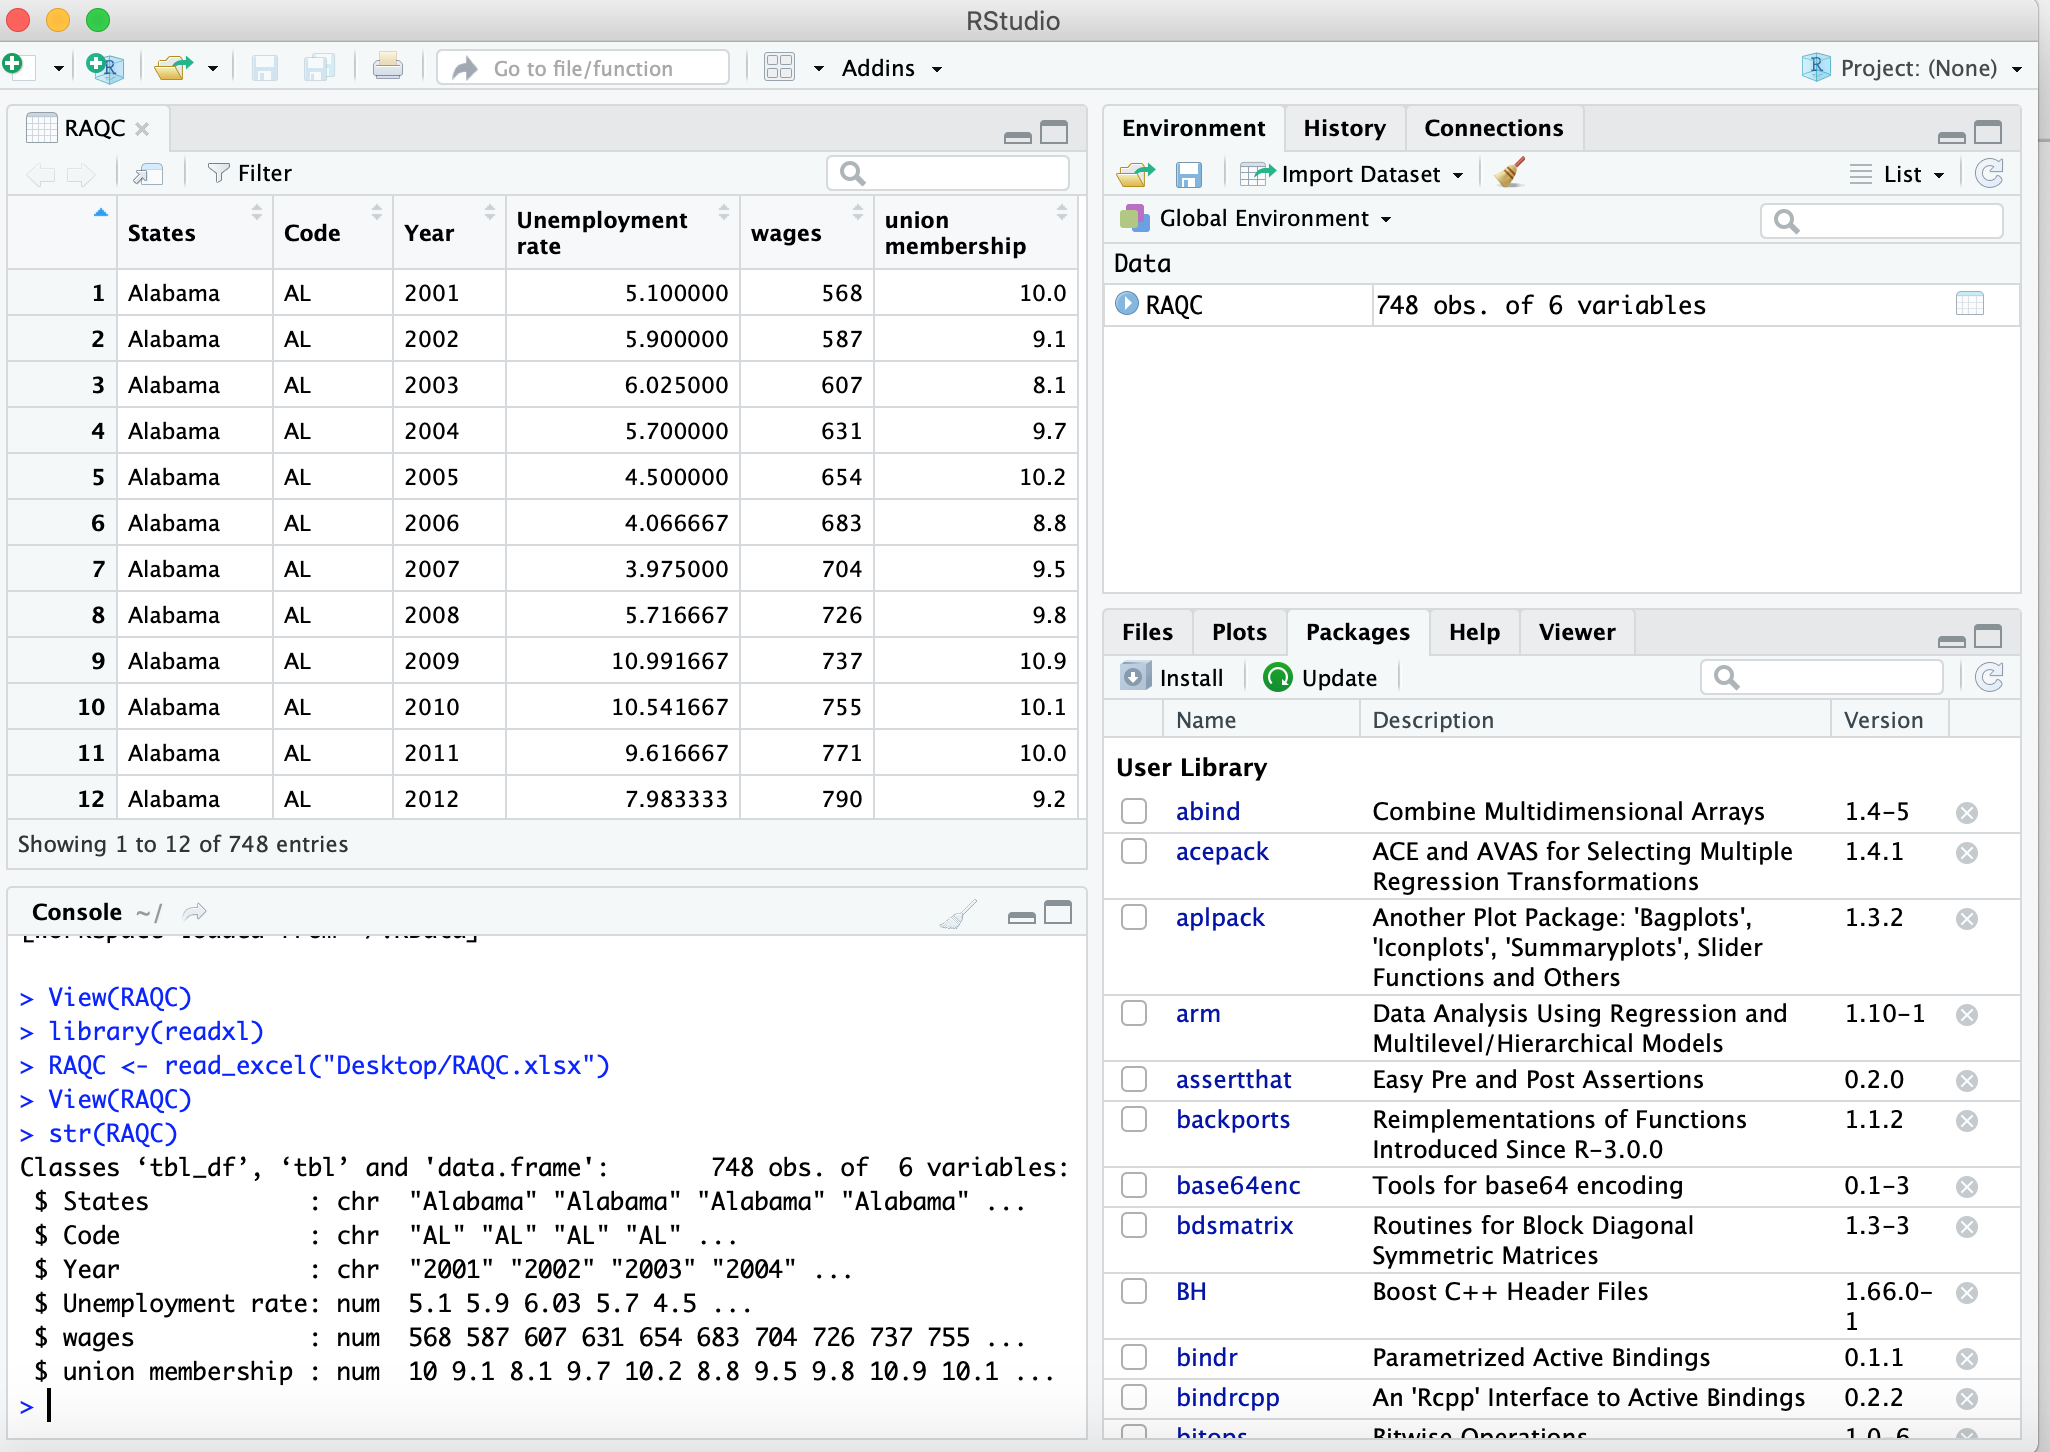
\includegraphics [width=7cm] {str.png} 
\end{center}
\end{frame}
\begin{frame}{\textbf{Cas pratique: syndicalisation et ch\^omage aux \'Etats-Unis}}
\setbeamercolor{block title}{use=structure,bg=noir,fg=white}
\setbeamercolor{block body}{use=structure,bg=ulor,fg=noir}
\begin{block}{Application du paquet plm}
\end{block}
Nous allons cr\'eer de nouvelles variables dans notre base de donn\'ees: 
\begin{enumerate}
\item  \'Etape 1: Cr\'eez une variable GFC, variable de contr\^ole pour la crise de 2008. 
\item  \'Etape 2: Cr\'eez des variables binaires de r\'egions (i.e.\ Nord-est, Sud, Mid-ouest, Ouest), variables de contr\^ole pour les r\'egions. 
\end{enumerate} 
\end{frame}
\begin{frame}{\textbf{Cas pratique: syndicalisation et ch\^omage aux \'Etats-Unis}}
\setbeamercolor{block title}{use=structure,bg=noir,fg=white}
\setbeamercolor{block body}{use=structure,bg=ulor,fg=noir}
\begin{block}{Application du paquet plm}
Notre  mod\`ele sera  sp\'ecifi\'e comme suit: 
   \begin{equation*}
lnChom_{it}= \beta_{1}lnSynd_{it}+ z_i \alpha +\beta_{2}GFC+\beta_{3}lnSal_{it}+u_{it}
    \end{equation*}
\end{block}
Avec i = 1, \ldots N et t = 1, \ldots T. \newline

O\`u $z_i $ contient un terme constant et les variables binaires de r\'egions (i.e.\ Mid-ouest, Sud, Ouest et Nord-est). \newline

\textbf{\textit{Rappel: pour \'eviter une multicolin\'earit\'e entre les variables binaires de r\'egions, n-1 r\'egions seront inclues dans le mod\`ele}}. 
\end{frame}
\begin{frame}{\textbf{Cas pratique: syndicalisation et ch\^omage aux \'Etats-Unis}}
\setbeamercolor{block title}{use=structure,bg=noir,fg=white}
\setbeamercolor{block body}{use=structure,bg=ulor,fg=noir}
\begin{block}{Application du paquet plm}
\end{block}
O\`u: 
\begin{description} 
 \item[lnChom repr\'esente l'\'evolution du taux de ch\^omage]
 \item[lnSynd repr\'esente l'\'evolution du taux de syndicalisation]
 \item[GFC repr\'esente la variable \textit{crise de 2008}]  
 \item[lnSal repr\'esente la croissance des salaires en pourcentage]
\end{description} 
\end{frame}
\begin{frame}{\textbf{Cas pratique: syndicalisation et ch\^omage aux \'Etats-Unis}}
\setbeamercolor{block title}{use=structure,bg=noir,fg=white}
\setbeamercolor{block body}{use=structure,bg=ulor,fg=noir}
\begin{block}{Application du paquet plm}
\end{block}
La d\'emarche de programmation avec R se fera durant l'atelier. \newline

Les codes utilis\'es pour ce cas pratique se trouvent dans l'annexe \textbf{\textit{Codes pour cas pratique \_ paquet plm}}. 
\end{frame}
\section{\textbf{Conclusion}}
\begin{frame}{\textbf{Conclusion}}
\setbeamercolor{block title}{use=structure,bg=noir,fg=white}
\setbeamercolor{block body}{use=structure,bg=ulor,fg=noir}
\begin{block}{Ce qu'il faut retenir!}
\end{block}
\begin{itemize}
\item Le paquet plm offre des outils int\'eressants pour faire une analyse de donn\'ees de panel avec R. 
\item Il existe plusieurs paquets qui permettent d'effectuer une analyse de donn\'ees de panel avec R (e.g.\ lme4 et nlme).
\item Cependant, l'int\'er\^et du paquet plm r\'eside dans le fait, \`a mon sens, qu'il s'adresse \`a des personnes famili\`eres avec le jargon de l'\'econom\'etrie ou qui s'inscrivent dans une approche \'econom\'etrique. 
\item Le paquet plm renferme des tests de sp\'ecification et d'autres tests utiles pour manipuler et analyser des donn\'ees de panel et pour en interpr\'eter les r\'esultats. 
\end{itemize}
\end{frame}
\section{\textbf{Bibliographie sommaire}}
\begin{frame}{\textbf{Bibliographie sommaire}}
\nocite{*} % adds all entries in the bib file to the bibliography
\printbibliography 
\end{frame}
\end{document}